%% This file was auto-generated by IPython, do NOT edit
%% Conversion from the original notebook file:
%% Fourier_Analysis.ipynb
%%
\documentclass[11pt,english]{article}

%% This is the automatic preamble used by IPython.  Note that it does *not*
%% include a documentclass declaration, that is added at runtime to the overall
%% document.

\usepackage{amsmath}
\usepackage{amssymb}
\usepackage{graphicx}
\usepackage{ucs}
\usepackage[utf8x]{inputenc}

% needed for markdown enumerations to work
\usepackage{enumerate}

% Slightly bigger margins than the latex defaults
\usepackage{geometry}
\geometry{verbose,tmargin=3cm,bmargin=3cm,lmargin=2.5cm,rmargin=2.5cm}

% Define a few colors for use in code, links and cell shading
\usepackage{color}
\definecolor{orange}{cmyk}{0,0.4,0.8,0.2}
\definecolor{darkorange}{rgb}{.71,0.21,0.01}
\definecolor{darkgreen}{rgb}{.12,.54,.11}
\definecolor{myteal}{rgb}{.26, .44, .56}
\definecolor{gray}{gray}{0.45}
\definecolor{lightgray}{gray}{.95}
\definecolor{mediumgray}{gray}{.8}
\definecolor{inputbackground}{rgb}{.95, .95, .85}
\definecolor{outputbackground}{rgb}{.95, .95, .95}
\definecolor{traceback}{rgb}{1, .95, .95}

% Framed environments for code cells (inputs, outputs, errors, ...).  The
% various uses of \unskip (or not) at the end were fine-tuned by hand, so don't
% randomly change them unless you're sure of the effect it will have.
\usepackage{framed}

% remove extraneous vertical space in boxes
\setlength\fboxsep{0pt}

% codecell is the whole input+output set of blocks that a Code cell can
% generate.

% TODO: unfortunately, it seems that using a framed codecell environment breaks
% the ability of the frames inside of it to be broken across pages.  This
% causes at least the problem of having lots of empty space at the bottom of
% pages as new frames are moved to the next page, and if a single frame is too
% long to fit on a page, will completely stop latex from compiling the
% document.  So unless we figure out a solution to this, we'll have to instead
% leave the codecell env. as empty.  I'm keeping the original codecell
% definition here (a thin vertical bar) for reference, in case we find a
% solution to the page break issue.

%% \newenvironment{codecell}{%
%%     \def\FrameCommand{\color{mediumgray} \vrule width 1pt \hspace{5pt}}%
%%    \MakeFramed{\vspace{-0.5em}}}
%%  {\unskip\endMakeFramed}

% For now, make this a no-op...
\newenvironment{codecell}{}

 \newenvironment{codeinput}{%
   \def\FrameCommand{\colorbox{inputbackground}}%
   \MakeFramed{\advance\hsize-\width \FrameRestore}}
 {\unskip\endMakeFramed}

\newenvironment{codeoutput}{%
   \def\FrameCommand{\colorbox{outputbackground}}%
   \vspace{-1.4em}
   \MakeFramed{\advance\hsize-\width \FrameRestore}}
 {\unskip\medskip\endMakeFramed}

\newenvironment{traceback}{%
   \def\FrameCommand{\colorbox{traceback}}%
   \MakeFramed{\advance\hsize-\width \FrameRestore}}
 {\endMakeFramed}

% Use and configure listings package for nicely formatted code
\usepackage{listingsutf8}
\lstset{
  language=python,
  inputencoding=utf8x,
  extendedchars=\true,
  aboveskip=\smallskipamount,
  belowskip=\smallskipamount,
  xleftmargin=2mm,
  breaklines=true,
  basicstyle=\small \ttfamily,
  showstringspaces=false,
  keywordstyle=\color{blue}\bfseries,
  commentstyle=\color{myteal},
  stringstyle=\color{darkgreen},
  identifierstyle=\color{darkorange},
  columns=fullflexible,  % tighter character kerning, like verb
}

% The hyperref package gives us a pdf with properly built
% internal navigation ('pdf bookmarks' for the table of contents,
% internal cross-reference links, web links for URLs, etc.)
\usepackage{hyperref}
\hypersetup{
  breaklinks=true,  % so long urls are correctly broken across lines
  colorlinks=true,
  urlcolor=blue,
  linkcolor=darkorange,
  citecolor=darkgreen,
  }

% hardcode size of all verbatim environments to be a bit smaller
\makeatletter 
\g@addto@macro\@verbatim\small\topsep=0.5em\partopsep=0pt
\makeatother 

% Prevent overflowing lines due to urls and other hard-to-break entities.
\sloppy

\begin{document}

\section{Fourier Analysis}

\subsection{Introduction}

In Fourier analysis, we take a complex periodic phenomenon apart,
decompose it into simpler parts. Then we assemble them in the form of
linear combination. Since we understand the simpler parts better, and we
know quite well how linear comnination works, we can expect to get a
better picture of the original phenomenon. This is a common strategy to
understand complicated things, called analysis and synthesis. But what
make Fourier analysis powerful is that we can implement the strategy
rigourously and effectively with the help of mathematical language.

A function $f$ with the property, $f(x + P) = f(x)$for every x, is
called a \textbf{periodic function}, and $P$ is the \textbf{period} of
the function. $sin$ and $cos$ are the simple periodic functions that are
going to be the building blocks of our analysis. Since
$sin(x + \frac{\pi}{2}) = cos(x)$, $sin$ and $cos$ are the same function
with different \textbf{phase}. Therefore, without losing any generality,
we can focus our study on the functions of the form $sin(x + \phi)$
where $\phi$ is the phase of the function.

Below are 4 sketches of $sin(x)$ graphs with different phases.

\begin{codecell}
\begin{codeinput}
\begin{lstlisting}
x = arange(0,2,0.01)
subplot(141)
title('$sin(2\pi x)$',size=20)
plot(x , sin(2*pi*x))
subplots_adjust(right = 2.3)
subplot(142)
title('$sin(2\pi x + \pi / 4)$',size=20)
plot(x, sin(2*pi*x+(pi/4)))
subplot(143)
title('$sin(2\pi x + \pi / 2) = cos(2\pi x)$',size=20)
plot(x, sin(2*pi*x+(pi/2)))
subplot(144)
title('$sin(2\pi x + \pi)$',size=20)
plot(x, sin(2*pi*x+(pi)))
\end{lstlisting}
\end{codeinput}
\begin{codeoutput}
\begin{verbatim}
[<matplotlib.lines.Line2D at 0xa1ac0d0>]
\end{verbatim}
\begin{center}
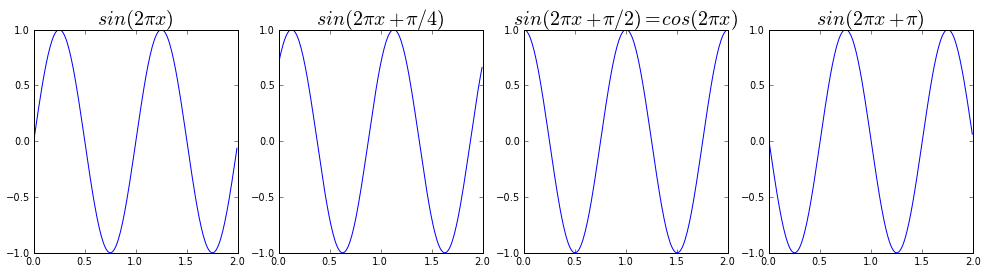
\includegraphics[width=6in]{Fourier_Analysis_files/Fourier_Analysis_fig_00.png}
\par
\end{center}
\end{codeoutput}
\end{codecell}
Besides \textbf{phases}, we can also change the \textbf{amplitudes},
\textbf{frequencies} of our functions. In short, our most general
building blocks are of the form $Asin(2 \pi ft + \phi)$, where $A$ is
the amplitude;$f$, the frequency. Finally we can form the sum:

\[\Sigma^n_1 A_k sin(2\pi f_k t + \phi_k)\]

To illustrate the fact that linear combination of simple trigonometric
functions can represent complicated function, we sketch the graphs of
the sum above, with different set of amplitude, frequency, and phase.

$sin(2\pi t) + sin(4\pi t) + sin(6\pi t)$

\begin{codecell}
\begin{codeinput}
\begin{lstlisting}
n = 200
domain = array([x])
one_vector = ones((1,n))
amplitude = array([[1,1,1]])
frequency = array([[1,2,3]])
phase = array([[0,0,0]])
y = sin(2*pi*domain.T.dot(frequency)+one_vector.T.dot(phase)).dot(amplitude.T)
plot(x,y)
\end{lstlisting}
\end{codeinput}
\begin{codeoutput}
\begin{verbatim}
[<matplotlib.lines.Line2D at 0xa4d3650>]
\end{verbatim}
\begin{center}
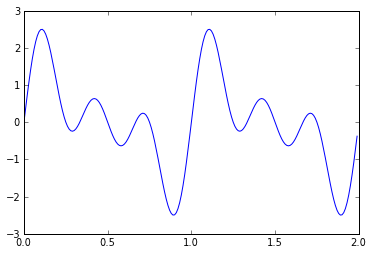
\includegraphics[width=6in]{Fourier_Analysis_files/Fourier_Analysis_fig_01.png}
\par
\end{center}
\end{codeoutput}
\end{codecell}
$sin(2\pi t) + sin(6\pi t) + sin(10\pi t) + sin(14\pi t) + sin(18\pi t) + sin(22\pi t)$

\begin{codecell}
\begin{codeinput}
\begin{lstlisting}
amplitude = array([[1,1,1,1,1,1]])
frequency = array([[1,3,5,7,9,11]])
phase = array([[0,0,0,0,0,0]])
y = sin(2*pi*domain.T.dot(frequency)+one_vector.T.dot(phase)).dot(amplitude.T)
plot(x,y)
\end{lstlisting}
\end{codeinput}
\begin{codeoutput}
\begin{verbatim}
[<matplotlib.lines.Line2D at 0xc4178d0>]
\end{verbatim}
\begin{center}
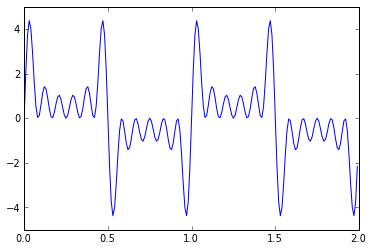
\includegraphics[width=6in]{Fourier_Analysis_files/Fourier_Analysis_fig_02.png}
\par
\end{center}
\end{codeoutput}
\end{codecell}
\begin{codecell}
\begin{codeinput}
\begin{lstlisting}
amplitude = array([[1,2,3,4,5,6,7]])
frequency = array([[2,3,5,7,11,13,17]])
phase = array([[0,0,0,0,0,0,0]])
y = sin(2*pi*domain.T.dot(frequency)+one_vector.T.dot(phase)).dot(amplitude.T)
plot(x,y)
\end{lstlisting}
\end{codeinput}
\begin{codeoutput}
\begin{verbatim}
[<matplotlib.lines.Line2D at 0xc836230>]
\end{verbatim}
\begin{center}
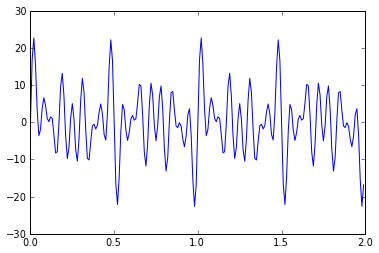
\includegraphics[width=6in]{Fourier_Analysis_files/Fourier_Analysis_fig_03.png}
\par
\end{center}
\end{codeoutput}
\end{codecell}

\begin{codecell}
\begin{codeinput}
\begin{lstlisting}
from traits.api import HasTraits,Array, Instance
from traitsui.api import View, Item
from chaco.api import HPlotContainer, ArrayPlotData, Plot
from enable.component_editor import ComponentEditor
\end{lstlisting}
\end{codeinput}
\end{codecell}
\begin{codecell}
\begin{codeinput}
\begin{lstlisting}
class sinsum(HasTraits):
    plot = Instance(Plot)
    traits_view = View(Item('plot',editor=ComponentEditor(), show_label=False),
                       width=1000, height=600, resizable=True, title="Chaco Plot")

    def __init__(self):
        super(sinsum, self).__init__()
        plotdata = ArrayPlotData(x = domain[0], y = sum_list_array(sin(2*pi*period.dot(domain))))
        img = Plot(plotdata)
        img.plot(("x","y"),type='line')
        self.plot = img
        return
        
\end{lstlisting}
\end{codeinput}
\end{codecell}

\end{document}
